\chapter{Project Management}
\label{app:project_management}
\section{Planning}
\subsection{Stakeholders}
This project can be appealing to a wide variety of Stakeholders. Firstly, the academic community
can be interested in the results to provide a new perspective of the influence of colors in users. 
It can also benefit the bursting internet industry where the user experience has become a key factor.
Given this knowledge, the project can be interesting for:
\begin{itemize}
    \item Psichology Researchers
    \item Human-Computer Interaction Researchers
    \item General Users
    \item Software Community and Students
    \item Private Companies that have a frontend product.
    \item Public Institutions 
\end{itemize}
\subsection{Organization Breakdown Structure (OBS) and Product Breakdown Structure (PBS)}
The OBS of the project as seen in figure \ref{fig:OBS} follows a hierarchical structure with three levels. 
Being the Project Manager the leader of this project and the one in charge of coordinating the software
engineer and the Lead Researcher. Secondly, the Lead Researcher is in charge of both junior researchers who
should be persons with knowledge in the field of computing and human computer interaction.
\begin{figure}[H]
    \centering
    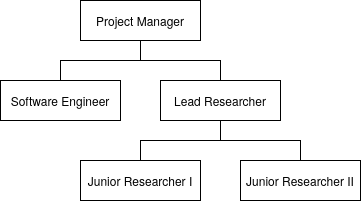
\includegraphics[width=0.7\textwidth]{figures/OBS.png}
    \caption{Organization Breakdown Structure (OBS)}
    \label{fig:OBS}
\end{figure}
There exists two main products which compose the Product Breakdown Structure (PBS) whcih then each of them have
different subtasks to develop them.
\begin{enumerate}
    \item \textbf{Experiment:} This is the main product where all the work is focused on. It is composed of three subtasks:
    \begin{enumerate}
        \item \textbf{Experiment Proposal:} The State of the Art and previous planning of the experiment.
        \item \textbf{Experiment Development:} The execution of the planned experiment.
        \item \textbf{Data Analysis:} The processing and analysis of the obtained data.
    \end{enumerate}
    \item \textbf{Documentation:} The final objective is to document the whole process into a scientific paper.
\end{enumerate}

The PBS described have a relation to the OBS as seen in table \ref{tab:rel_OBS_PBS}.
\begin{table}[H]
    \centering
    \caption{Relation between OBS and PBS}
    \label{tab:rel_OBS_PBS}
    \begin{tabularx}{\textwidth}{|>{\raggedright\arraybackslash}X|>{\raggedright\arraybackslash}X|>{\raggedright\arraybackslash}X|}
        \hline
        \textbf{Task} & \textbf{Resource} & \textbf{Product} \\
        \hline
        \textbf{State of the Art} & Junior Researchers, Lead Researcher & Experiment Proposal \\
        \hline
        \textbf{Previous Planning} & Project Manager, Lead Researcher & Experiment Proposal \\
        \hline
        \textbf{Experiment Planning} & Software Engineer, Lead Researcher & Experiment Development \\
        \hline
        \textbf{Experiment Execution} & Junior Researchers & Experiment Development \\
        \hline
        \textbf{Tobii Preparations} & Software Engineer & Experiment Development \\
        \hline
        \textbf{Data Preprocessing} & Software Engineer, Junior Researchers & Data Analysis \\
        \hline
        \textbf{Data Processing} & Software Engineer & Data Analysis \\
        \hline
        \textbf{Statistical Study} & Lead Resercher & Data Analysis \\
        \hline
        \textbf{Paper Writing} & Junior Researchers & Documentation \\
        \hline
        \textbf{Paper Review} & Lead Researcher  & Documentation \\
        \hline
    \end{tabularx}
\end{table}
\section{Risk Identification and Management}
Risk identification is a key phase of the project as it can help acknowledge possible negative 
effects on the project. It is important to have a strategy to face such events in order to make 
them affect the least possible the outcome of the project.
\begin{table} [H]
    \centering
    \caption{Risks List}
    \label{tab:risks}
    \begin{tabularx}{0.8\textwidth} { 
        | >{\raggedright\arraybackslash}c 
        | >{\centering\arraybackslash}X| }
        \hline \textbf{Risk ID} & \textbf{Risk Name} \\
        \hline
        \textbf{1} & Few Experimental Samples \\
        \hline
        \textbf{2} & Statistical Analysis Imprecision \\
        \hline
        \textbf{3} & Loss of Partial Work \\
        \hline
        \textbf{4} & Justified Leave of Worker \\
        \hline
        \textbf{5} & Lack of Teamwork \\
        \hline
        \textbf{6} & Tobii Measurements Drifts \\
        \hline
        \textbf{7} & Privacy Violations \\
        \hline
        \textbf{8} & Timeline Delay \\
        \hline
        \textbf{9} & Publisher Rejection \\
        \hline
    \end{tabularx}
\end{table}
\subsection{Risk Details}
\label{sub:risk_details}
\subsubsection{Few Experimental Samples}
There is not enough sample for the test, this can lead to inconsistent
 data and problems when doing the processing and publishing the paper.
\begin{table}[H]
    \centering
    \small
    \renewcommand{\arraystretch}{1.8}
    \setlength{\tabcolsep}{3pt} 
    
    \caption{Few experimental samples impact.}
    \label{tab:risk_impact}
    
    \begin{tabularx}{\textwidth}
        {|>{\centering\arraybackslash}X|>{\centering\arraybackslash}X|>{\centering\arraybackslash}X|>
        {\centering\arraybackslash}X|>{\centering\arraybackslash}X|>{\centering\arraybackslash}p{1.5cm}|}
        \hline
        \multirow{2}{*}{\textbf{Probability}} & \multicolumn{4}{c|}{\textbf{Impact}} 
        & \multirow{2}{*}{\textbf{Impact}} \\ \cline{2-5}
        
        & \textbf{Budget} & \textbf{Planning} & \textbf{Reach} & \textbf{Quality} & \\ \hline
        
        Medium & Low & Low & Medium & Critic & \cellcolor{orange} 0,45 \\ \hline
    \end{tabularx}
\end{table}
\subsubsection{Statistical Analysis Imprecision}
When analyzing the processed data if the statistic analysis is imprecise it can lead to wrong 
conclusions. It is important for it to remain precise.
\begin{table} [H]
    \centering
    \small
    \renewcommand{\arraystretch}{1.8}
    \setlength{\tabcolsep}{3pt} 
    
    \caption{Statistical analysis imprecision impact.}
    \label{tab:risk_impact2}
    
    \begin{tabularx}{\textwidth}
        {|>{\centering\arraybackslash}X|>{\centering\arraybackslash}X|>{\centering\arraybackslash}X|>
        {\centering\arraybackslash}X|>{\centering\arraybackslash}X|>{\centering\arraybackslash}p{1.5cm}|}
        \hline
        \multirow{2}{*}{\textbf{Probability}} & \multicolumn{4}{c|}{\textbf{Impact}} 
        & \multirow{2}{*}{\textbf{Impact}} \\ \cline{2-5}
        
        & \textbf{Budget} & \textbf{Planning} & \textbf{Reach} & \textbf{Quality} & \\ \hline
        
        Low & Seamless & Low & Low & Medium & \cellcolor{green!40} 0,09 \\ \hline
    \end{tabularx}
\end{table}
\subsubsection{Loss of Partial Work}
Due to data corruption or any other external agent, there’s a possibility of losing the entire 
or part of the work accomplished.
\begin{table}[H]
    \centering
    \small
    \renewcommand{\arraystretch}{1.8}
    \setlength{\tabcolsep}{3pt} 
    
    \caption{Loss of partial work impact.}
    \label{tab:risk_impact3}
    
    \begin{tabularx}{\textwidth}
        {|>{\centering\arraybackslash}X|>{\centering\arraybackslash}X|>{\centering\arraybackslash}X|>
        {\centering\arraybackslash}X|>{\centering\arraybackslash}X|>{\centering\arraybackslash}p{1.5cm}|}
        \hline
        \multirow{2}{*}{\textbf{Probability}} & \multicolumn{4}{c|}{\textbf{Impact}} 
        & \multirow{2}{*}{\textbf{Impact}} \\ \cline{2-5}
        
        & \textbf{Budget} & \textbf{Planning} & \textbf{Reach} & \textbf{Quality} & \\ \hline
        
        Low & Medium & High & Medium & Low & \cellcolor{green!40} 0,17 \\ \hline
    \end{tabularx}
\end{table}
\subsubsection{Justified Leave of Worker}
Any of the workers may need a justified leave of work according to the Spanish law.
\begin{table}[H]
    \centering
    \small
    \renewcommand{\arraystretch}{1.8}
    \setlength{\tabcolsep}{3pt} 
    
    \caption{Justified leave of worker impact.}
    \label{tab:risk_impact4}
    
    \begin{tabularx}{\textwidth}
        {|>{\centering\arraybackslash}X|>{\centering\arraybackslash}X|>{\centering\arraybackslash}X|>
        {\centering\arraybackslash}X|>{\centering\arraybackslash}X|>{\centering\arraybackslash}p{1.5cm}|}
        \hline
        \multirow{2}{*}{\textbf{Probability}} & \multicolumn{4}{c|}{\textbf{Impact}} 
        & \multirow{2}{*}{\textbf{Impact}} \\ \cline{2-5}
        
        & \textbf{Budget} & \textbf{Planning} & \textbf{Reach} & \textbf{Quality} & \\ \hline
        
        Medium & Low & High & Low & Low & \cellcolor{yellow} 0,28 \\ \hline
    \end{tabularx}
\end{table}
\subsubsection{Lack of Teamwork}
Teamwork is important as it creates a healthy environment where workers feel comfortable, 
however it is quite easy to have a lot of individualism in teams.
\begin{table} [H]
    \centering
    \small
    \renewcommand{\arraystretch}{1.8}
    \setlength{\tabcolsep}{3pt} 
    
    \caption{Lack of teamwork impact.}
    \label{tab:risk_impact5}
    
    \begin{tabularx}{\textwidth}
        {|>{\centering\arraybackslash}X|>{\centering\arraybackslash}X|>{\centering\arraybackslash}X|>
        {\centering\arraybackslash}X|>{\centering\arraybackslash}X|>{\centering\arraybackslash}p{1.5cm}|}
        \hline
        \multirow{2}{*}{\textbf{Probability}} & \multicolumn{4}{c|}{\textbf{Impact}} 
        & \multirow{2}{*}{\textbf{Impact}} \\ \cline{2-5}
        
        & \textbf{Budget} & \textbf{Planning} & \textbf{Reach} & \textbf{Quality} & \\ \hline
        
        Medium & Low & High & Low & Low & \cellcolor{green!40} 0,15 \\ \hline
    \end{tabularx}
\end{table}
\subsubsection{Tobii Measurements Drifts}
Due to light changes, the subject of the experiment looking away or other uncontrollable 
events, the tobii eye-tracker may drift its measurements.
\begin{table} [H]
    \centering
    \small
    \renewcommand{\arraystretch}{1.8}
    \setlength{\tabcolsep}{3pt} 
    
    \caption{Tobii measurements drifts impact.}
    \label{tab:risk_impact6}
    
    \begin{tabularx}{\textwidth}
        {|>{\centering\arraybackslash}X|>{\centering\arraybackslash}X|>{\centering\arraybackslash}X|>
        {\centering\arraybackslash}X|>{\centering\arraybackslash}X|>{\centering\arraybackslash}p{1.5cm}|}
        \hline
        \multirow{2}{*}{\textbf{Probability}} & \multicolumn{4}{c|}{\textbf{Impact}} 
        & \multirow{2}{*}{\textbf{Impact}} \\ \cline{2-5}
        
        & \textbf{Budget} & \textbf{Planning} & \textbf{Reach} & \textbf{Quality} & \\ \hline
        
        High & Seamless & Seamless & Seamless & Medium & \cellcolor{yellow} 0,21 \\ \hline
    \end{tabularx}
\end{table}
\subsubsection{Privacy Violations}
This whole research gathers a lot of sensitive information and it is a key to store and 
manipulate the sensitive data correctly as it can lead to fines.
\begin{table} [H]
    \centering
    \small
    \renewcommand{\arraystretch}{1.8}
    \setlength{\tabcolsep}{3pt} 
    
    \caption{Privacy violations impact.}
    \label{tab:risk_impact7}
    
    \begin{tabularx}{\textwidth}
        {|>{\centering\arraybackslash}X|>{\centering\arraybackslash}X|>{\centering\arraybackslash}X|>
        {\centering\arraybackslash}X|>{\centering\arraybackslash}X|>{\centering\arraybackslash}p{1.5cm}|}
        \hline
        \multirow{2}{*}{\textbf{Probability}} & \multicolumn{4}{c|}{\textbf{Impact}} 
        & \multirow{2}{*}{\textbf{Impact}} \\ \cline{2-5}
        
        & \textbf{Budget} & \textbf{Planning} & \textbf{Reach} & \textbf{Quality} & \\ \hline
        
        Low & Critic & Low & Seamless & Low & \cellcolor{yellow} 0,27 \\ \hline
    \end{tabularx}
\end{table}
\subsubsection{Timeline Delay}
Research projects usually take longer than initially expected this can overextend the planning making it a real risk.
\begin{table} [H]
    \centering
    \small
    \renewcommand{\arraystretch}{1.8}
    \setlength{\tabcolsep}{3pt} 
    
    \caption{Timeline delay impact.}
    \label{tab:risk_impact8}
    
    \begin{tabularx}{\textwidth}
        {|>{\centering\arraybackslash}X|>{\centering\arraybackslash}X|>{\centering\arraybackslash}X|>
        {\centering\arraybackslash}X|>{\centering\arraybackslash}X|>{\centering\arraybackslash}p{1.5cm}|}
        \hline
        \multirow{2}{*}{\textbf{Probability}} & \multicolumn{4}{c|}{\textbf{Impact}} 
        & \multirow{2}{*}{\textbf{Impact}} \\ \cline{2-5}
        
        & \textbf{Budget} & \textbf{Planning} & \textbf{Reach} & \textbf{Quality} & \\ \hline
        
        High & High & High & Medium & Low & \cellcolor{YellowOrange} 0,39 \\ \hline
    \end{tabularx}
\end{table}
\subsubsection{Publisher Rejection}
After finishing the experiment, gathering the data and writing the paper there’s a 
possibility the desired scientific publishers may not be interested in the paper.
\begin{table} [H]
    \centering
    \small
    \renewcommand{\arraystretch}{1.8}
    \setlength{\tabcolsep}{3pt} 
    
    \caption{Publisher rejection impact.}
    \label{tab:risk_impact9}
    
    \begin{tabularx}{\textwidth}
        {|>{\centering\arraybackslash}X|>{\centering\arraybackslash}X|>{\centering\arraybackslash}X|>
        {\centering\arraybackslash}X|>{\centering\arraybackslash}X|>{\centering\arraybackslash}p{1.5cm}|}
        \hline
        \multirow{2}{*}{\textbf{Probability}} & \multicolumn{4}{c|}{\textbf{Impact}} 
        & \multirow{2}{*}{\textbf{Impact}} \\ \cline{2-5}
        
        & \textbf{Budget} & \textbf{Planning} & \textbf{Reach} & \textbf{Quality} & \\ \hline
        
        High & Seamless & Low & High & Low & \cellcolor{YellowOrange} 0,39 \\ \hline
    \end{tabularx}
\end{table}

\subsection{Risk Strategy}
A risk strategy is needed in order to know what to do against every risk, the risks of 
\ref{sub:risk_details} explains them further. From the 9 identified risks, 2 will be deleted, 3 assumed and 4 mitigated.
\begin{table} [H]
    \centering
    \small
    \caption{Risk strategy and action plan.}
    \label{tab:risk_strategy}
    \setlength{\tabcolsep}{4pt}
    
    
    \begin{tabularx}{\textwidth} { 
        | c % ID
        | >{\raggedright\arraybackslash}X % Risk Name
        | c % Impact
        | c % Strategy
        | >{\raggedright\arraybackslash}p{6cm} | 
    }
        \hline 
        \textbf{ID} & \textbf{Risk Name} & \textbf{Impact} & \textbf{Strategy} & \textbf{Risk Answer}\\
        \hline
        \textbf{1} & Few Experimental Samples & \cellcolor{orange} 0,45 & Delete & Spend more time than planned gathering samples for the experiment. \\ \hline
        \textbf{8} & Timeline Delay & \cellcolor{YellowOrange} 0,39 & Mitigate & When creating the planning always adding more time than expected. \\ \hline
        \textbf{9} & Publisher Rejection & \cellcolor{YellowOrange} 0,39 & Assume & It should be necessary to have a broad list of publishers. \\ \hline
        \textbf{4} & Justified Leave of Worker & \cellcolor{yellow} 0,28 & Assume & Work the planning around the person missing. \\ \hline    
        \textbf{7} & Privacy Violations & \cellcolor{yellow} 0,27 & Delete & Exhaustive analysis by the prepared workers on the RGPD. \\ \hline
        \textbf{6} & Tobii Measurements Drifts & \cellcolor{yellow} 0,21 & Assume & Try to find a spot with balanced lighting. \\ \hline
        \textbf{3} & Loss of Partial Work & \cellcolor{green!40} 0,17 & Mitigate & Integrate a version control system on the work. \\ \hline
        \textbf{5} & Lack of Teamwork & \cellcolor{green!40} 0,15 & Mitigate & Weekly optional team buildings outside of the work period. \\ \hline
        \textbf{2} & Statistical Analysis Imprecision & \cellcolor{green!40} 0,09 & Mitigate & Final deep review of the statistical analysis. \\ \hline
    \end{tabularx}
\end{table}
\newpage
\section{Incidence Log}
The incidence log is a document where incidents are described with their date. It serves as a way to understand and keep
track of the incidents that happen during the project.
\begin{table} [H]
    \centering
    \small
    \caption{Incidence log.}
    \label{tab:incidence_log}
    \setlength{\tabcolsep}{4pt}
    
    \begin{tabularx}{\textwidth} { 
        | c 
        | >{\raggedright\arraybackslash}X 
        | >{\raggedright\arraybackslash}X | 
    }
        \hline 
        \textbf{Date} & \textbf{Incident Description} & \textbf{Solution} \\ \hline
        \textbf{17/10/2024} & Lack of availability in scientific websites & After contacting the professors, it was possible
        to find scientific paper searchers. \\ \hline
        \textbf{24/04/2025} & Lack of participants for the experiment & Bringing known colleagues helped gathering data and creating
        inertia to gather more participants. \\ \hline
        \textbf{18/05/2025} & Documentation and Tobii Data Loss & Version control was established and the latest available version was restored. \\ \hline
        \textbf{27/05/2025} & Project delay & Due to not enough availaiblity the problem was solved by extending to next year the deadline of the project. \\ \hline
        \textbf{12/11/2025} & Problems with titles and table of contents & After hard work, the documentation was moved from word to latex. \\ \hline
    \end{tabularx}
\end{table}